% TFF-Title: EPC query and acknowledgement loop
% TFF-Family: flowchart
% TFF-Tags: flowchart, epc, state-machine, feedback-loop, orthogonal-routing
% TFF-Description: Four-state EPC flow with generous spacing, explicit conditions, and non-overlapping feedback routes.
% TFF-Origin: https://texample.net/epc-flow-charts/
% TFF-License: CC BY-SA 4.0
% TFF-Attribution: Adapted from Fabian Schuh's EPC flow charts example on TeXample.net
\documentclass[tikz,border=8pt]{standalone}
\usetikzlibrary{arrows.meta,positioning}
\begin{document}
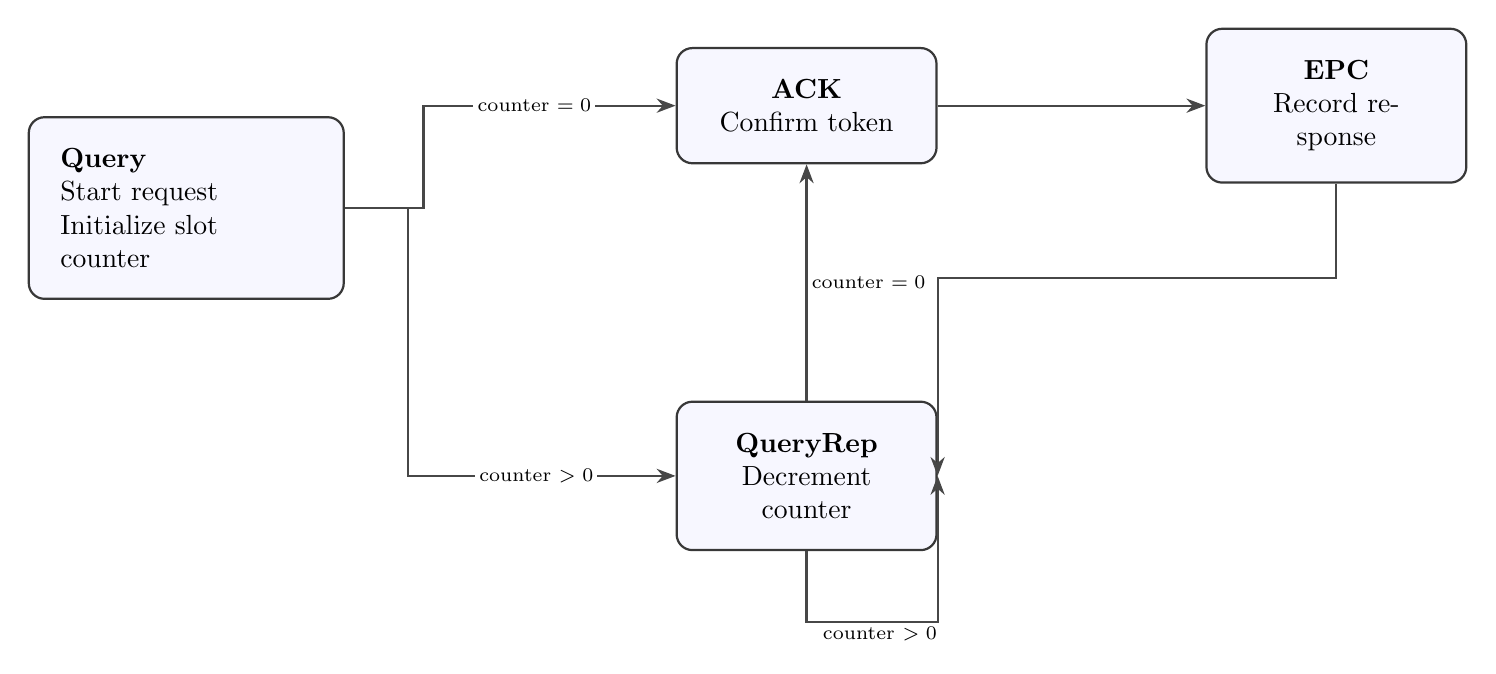
\begin{tikzpicture}[
  state/.style={rounded corners=2mm,draw=black!78,line width=.8pt,
    fill=blue!3,minimum height=12mm,text width=32mm,align=left,inner sep=4mm},
  compact/.style={state,text width=25mm,align=center},
  flow/.style={-{Stealth[length=2.4mm]},draw=black!72,line width=.8pt},
  labelbox/.style={fill=white,inner sep=1.5pt,font=\scriptsize,align=center}
]
\node[state] (query) {\textbf{Query}\\Start request\\Initialize slot counter};
\node[compact,right=42mm of query,yshift=13mm] (ack) {\textbf{ACK}\\Confirm token};
\node[compact,below=30mm of ack] (rep) {\textbf{QueryRep}\\Decrement counter};
\node[compact,right=34mm of ack] (epc) {\textbf{EPC}\\Record response};
\draw[flow] (query.east) -- ++(10mm,0) |- node[labelbox,pos=.72] {counter $=0$} (ack.west);
\draw[flow] (query.east) -- ++(8mm,0) |- node[labelbox,pos=.74] {counter $>0$} (rep.west);
\draw[flow] (ack.east) -- (epc.west);
\draw[flow] (rep.north) -- node[labelbox,right] {counter $=0$} (ack.south);
\draw[flow] (rep.south) -- ++(0,-9mm) -| node[labelbox,pos=.28,below] {counter $>0$} (rep.east);
\draw[flow] (epc.south) -- ++(0,-12mm) -| (rep.east);
\end{tikzpicture}
\end{document}
